\documentclass[a4paper]{article}
\usepackage{graphicx}
\usepackage{amsmath,amssymb}
\usepackage{hyperref}
\usepackage{minted}
\usepackage{multirow}
\usepackage{float}
\usepackage{todonotes}
\usepackage{forest}
\usepackage{xstring}
\title{Action potential / Spike}
\date{}


\begin{document}
    \url{https://en.wikipedia.org/wiki/Action_potential}
    Also called as spike
    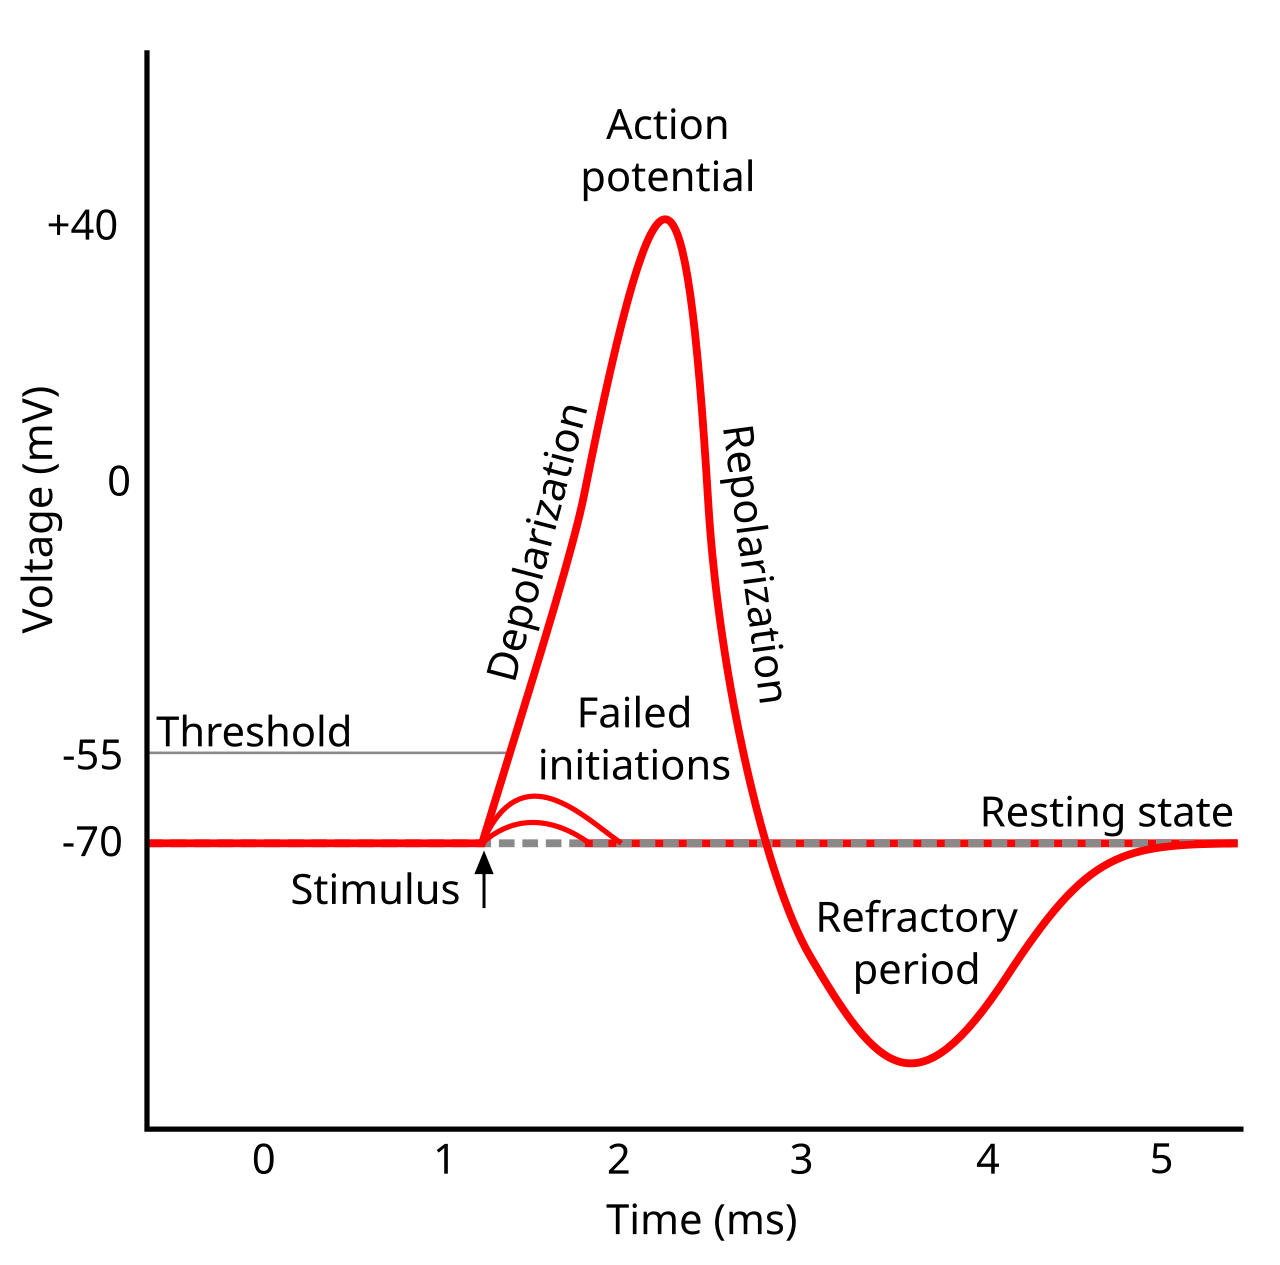
\includegraphics[width=\paperwidth]{action_potential.png}
    
    
    \section{Spike train}
        The temporal sequence of action potentials generated by a neuron is called its ``spike train``
\end{document}
